\documentclass{article}
\usepackage{graphicx}
\usepackage{longtable}
\usepackage{hyperref}
\usepackage{enumitem}
\usepackage{geometry}
\usepackage{amsmath}
\usepackage{amssymb}
\usepackage{listings}
\usepackage{physics}
\usepackage{booktabs}
\usepackage{array}
\geometry{a4paper, margin=1in}

\begin{document}
\title{\texttt{MATLAB} Scientific Calculator on \texttt{Python}}
\author{George Huang}
\date{\today}
\maketitle

\begin{center}
\noindent{THE UNIVERSITY OF HONG KONG}

\noindent{DEPARTMENT OF MATHEMATICS}
\end{center}

\begin{figure}[h]
\centering
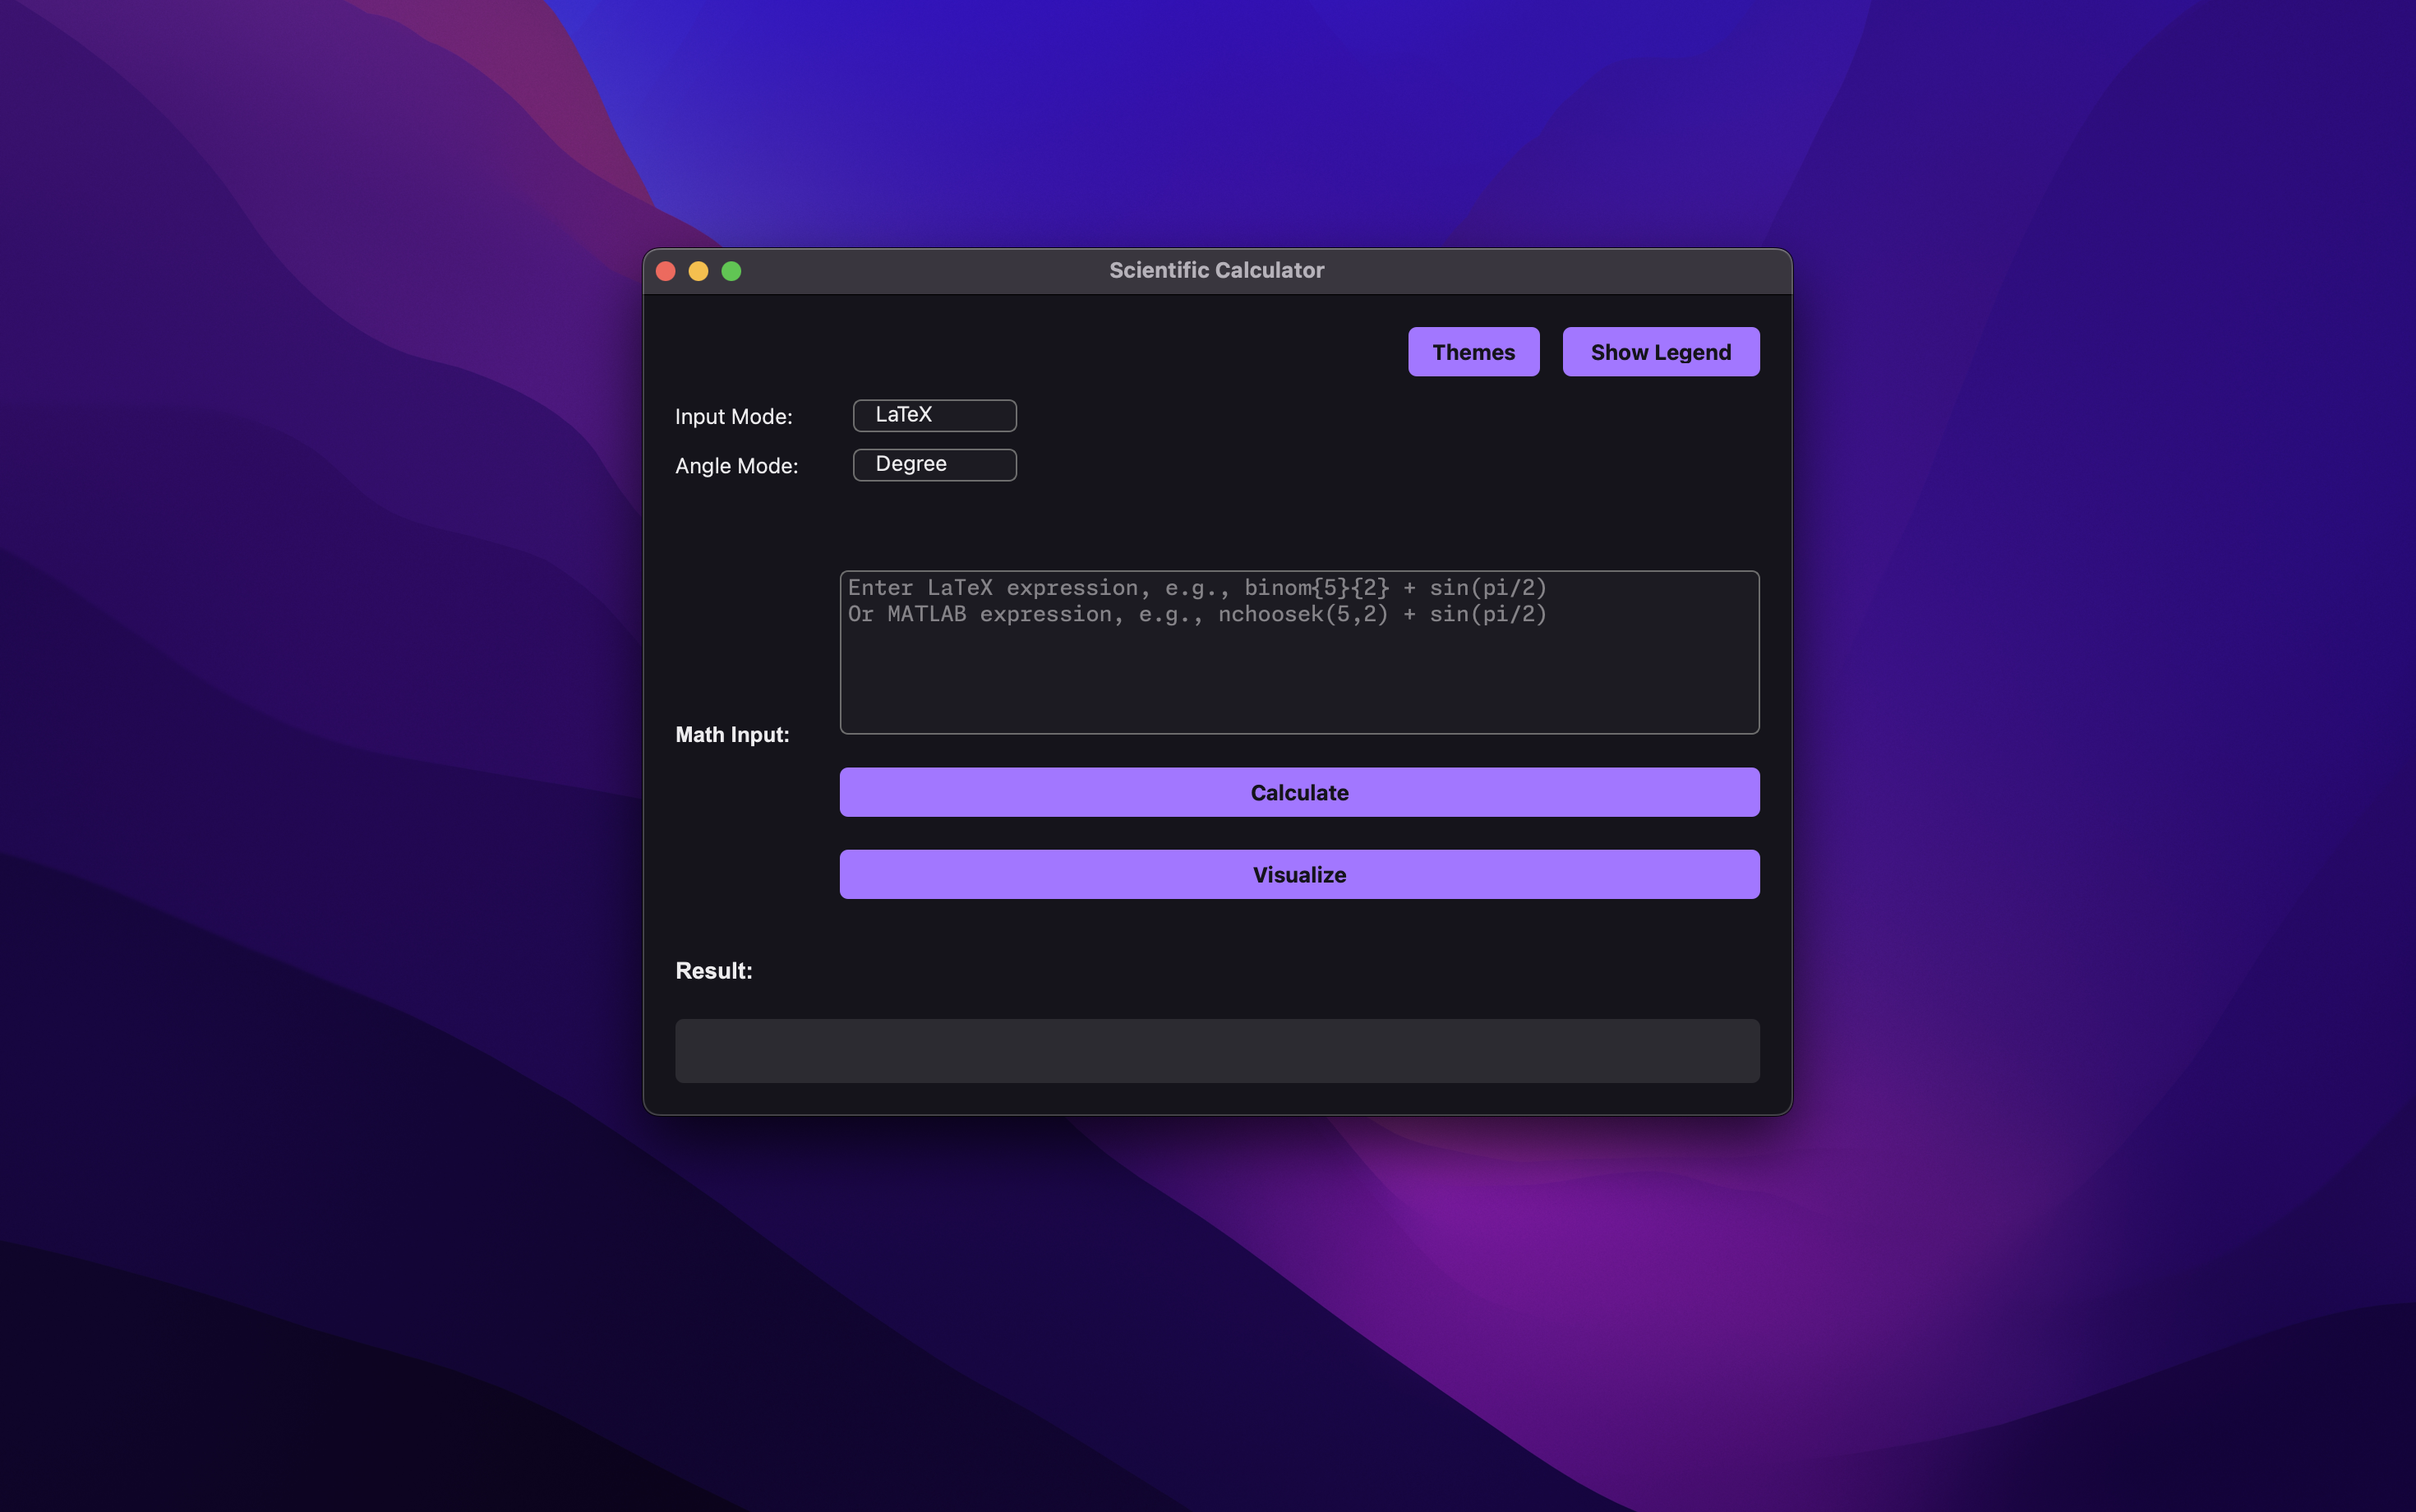
\includegraphics[width=\linewidth]{imgs/legend_img.png}
\caption{legend img}
\end{figure}

\section{Introduction}

\noindent A \texttt{PyQt5}-based scientific calculator that supports \LaTeX \, input,
integrates with \texttt{MATLAB} for symbolic computation, and offers various
mathematical functionalities including differentiation, integration, and
matrix operations.

\subsection{Features}

\begin{itemize}
\item \LaTeX \, Input: Enter mathematical expressions in
  \LaTeX \, format for easy readability and input.
\item \texttt{MATLAB} Integration: Utilize \texttt{MATLAB}'s symbolic toolbox for
  advanced computations, ensuring high precision and reliability.
\item Trigonometric Functions: Supports both Degree and Radian
  modes for trigonometric calculations.
\item Symbolic Computation: Handle derivatives and integrals
  symbolically, providing exact results where possible.
\item Matrix Operations: Perform operations such as determinant,
  inverse, eigenvalues, and more on matrices.
\item Theming: Multiple UI themes available to customize the
  appearance of the application.
\item Logging: Detailed logging of operations and errors for
  troubleshooting and analysis.
\item Auto Simplify: Automatically simplifies the result of the
  expression.
\end{itemize}

\hfill

\subsection{Getting Started}

\noindent

\begin{enumerate}
\def\labelenumi{\arabic{enumi}.}
\item Clone the Repository:

\begin{verbatim}
    git clone https://github.com/Goge052215/MATLAB-Calculator-on-py.git
\end{verbatim}

\item Install Required Fonts:

  Thanks for developers of Monaspace font family! We are using the font
  \href{https://monaspace.githubnext.com/}{\textit{Monaspace Neon}} for
  the UI (partially).You can install the font by running the scripts in
  \url{fonts} folder.

  So far, there are 2 scripts for following systems:

  \begin{itemize}
  \item \href{https://github.com/Goge052215/MATLAB-Calculator-on-py/blob/master/fonts/fonts_download.ps1}{\texttt{Windows}}
  \item \href{https://github.com/Goge052215/MATLAB-Calculator-on-py/blob/master/fonts/fonts_download.bash}{\texttt{MacOS}}
  \end{itemize}

  \noindent For \texttt{Linux} users, please see the instructions in the
  \href{https://github.com/githubnext/monaspace?tab=readme-ov-file}{GitHub
  Monaspace repository}.

\item Install Dependencies:

  \noindent Ensure you have \texttt{MATLAB} installed and the \texttt{MATLAB} Engine API for \texttt{Python}
  set up.

\begin{verbatim}
    pip install -r requirements.txt
\end{verbatim}

  \noindent The requirement list is in \href{https://github.com/Goge052215/MATLAB-Calculator-on-py/blob/master/requirements.txt}{\texttt{requirements.txt}}

\item Run the Application:

\begin{verbatim}
    python main.py
\end{verbatim}
\end{enumerate}

\subsection{Usage}

\begin{enumerate}
\def\labelenumi{\arabic{enumi}.}
\item Select Input Mode:

  \begin{itemize}
  \item \LaTeX: Enter expressions in \LaTeX \, format for symbolic computation.
  \item \texttt{MATLAB}: Enter raw \texttt{MATLAB} expressions for direct evaluation.
  \item Matrix: Perform matrix operations (e.g., determinant, inverse).
  \end{itemize}

\item Select Angle Mode:

  \begin{itemize}
  \item Degree: Use degree mode for trigonometric functions.
  \item Radian: Use radian mode for trigonometric functions.
  \end{itemize}

\item Enter Expression:

  \begin{itemize}
  \item In the input field, type your mathematical expression.
  \end{itemize}

\item Calculate:

  \begin{itemize}
  \item Click the ``Calculate'' button to evaluate the expression.
  \end{itemize}

\item View Result:

  \begin{itemize}
  \item The result will be displayed below the calculate button.
  \end{itemize}
\end{enumerate}

\subsection{Example Expressions}

\noindent

\begin{itemize}
\item Simplified \LaTeX \, Mode:

  \begin{itemize}
  \item Differentiation: \texttt{d/dx\ (x\^{}2)},
    \texttt{d2/dx2\ (x\^{}2)}, etc.
  \item Integration: \texttt{int\ e\^{}(x)\ dx},
    \texttt{int\ ln(x)\ dx}, \texttt{int\ x\^{}2\ dx}, etc.
  \item Trigonometric: \texttt{sin(30)}, \texttt{cos(30)},
    \texttt{tan(30)}, etc.
  \end{itemize}
\item
  \texttt{MATLAB} Mode:

  \begin{itemize}
  \item Differentiation: \texttt{diff(x\^{}2,\ x)},
    \texttt{diff(x\^{}2,\ x,\ 2)}, etc.
  \item Integration: \texttt{int (exp(x),\ x)},
    \texttt{int (ln(x),\ x)}, \texttt{int (x\^{}2,\ x)}, etc.
  \item Trigonometric: \texttt{sin (30)}, \texttt{cos (30)},
    \texttt{tan (30)}, etc.
  \end{itemize}
\end{itemize}

\noindent

\noindent \emph{Note:} Simplified \LaTeX \, input is recommended, for a guide of
simplified \LaTeX \, input, see the table below:

\renewcommand{\arraystretch}{2.2}

\begin{longtable}[]{@{}
  >{\raggedright\arraybackslash}p{0.20\linewidth}
  >{\raggedright\arraybackslash}p{0.35\linewidth}
  >{\raggedright\arraybackslash}p{0.35\linewidth}@{}}
\toprule
\begin{minipage}[b]{\linewidth}\raggedright
\LaTeX
\end{minipage} & \begin{minipage}[b]{\linewidth}\raggedright
Previous \LaTeX \, Command
\end{minipage} & \begin{minipage}[b]{\linewidth}\raggedright
Simplified \LaTeX \, Input
\end{minipage} \\
\midrule
\endhead
\(\displaystyle\frac{\dd}{\dd x}(f(x))\) &
\texttt{\textbackslash{}frac\{d\}\{dx\}\ (f(x))} &
\texttt{d/dx\ (f(x))} \\
\(\displaystyle\frac{\dd[n]}{\dd[n]x}(f(x))\) &
\texttt{\textbackslash{}frac\{d\^{}n\}\{dx\^{}n\}\ (f(x))} &
\texttt{dn/dxn\ (f(x))} \\
\(\displaystyle\int e^{x} \, \dd x\) &
\texttt{\textbackslash{}int\ e\^{}\{x\}\ dx} &
\texttt{int\ e\^{}x\ dx} \\
\(\displaystyle\int_{a}^{b} f(x) \, \dd x\) &
\texttt{\textbackslash{}int\_\{a\}\^{}\{b\}\ f(x)\ dx} &
\texttt{int\ (a\ to\ b)\ f(x)\ dx} \\
\(\sin, \cos, \tan, \dots\) &
\texttt{\textbackslash{}sin,\ \textbackslash{}cos,\ \textbackslash{}tan,\ ...}
& \texttt{sin,\ cos,\ tan,\ ...} \\
\(\displaystyle\binom{n}{r}\) or \(^n\text{C}_r\) &
\texttt{\textbackslash{}binom\{n\}\{r\}} & \texttt{binom(n,\ r)} \\
\(\sqrt{x}\) & \texttt{\textbackslash{}sqrt\{x\}} & \texttt{sqrt(x)} \\
\(\abs{x}\) &
\texttt{\textbackslash{}abs\{x\}} &
\texttt{abs(x)} \\
\(\ln(x)\) & \texttt{\textbackslash{}ln(x)} & \texttt{ln(x)} \\
\(\log_{10}(x)\) & \texttt{\textbackslash{}log\_\{10\}(x)} &
\texttt{log10(x)} \\
\(\log_{n}(x)\) & \texttt{\textbackslash{}log\_\{n\}(x)} &
\texttt{logn(x)} \\
\(\alpha, \beta, \gamma, \dots\) &
\texttt{\textbackslash{}alpha,\ \textbackslash{}beta,\ \textbackslash{}gamma,\ ...}
& \texttt{alpha,\ beta,\ gamma,\ ...} \\
\(\displaystyle\sum_{i = a}^{b-a} f(x_i)\) &
\texttt{\textbackslash{}sum\_\{i\ =\ a\}\^{}\{b-a\}\ f(x\_i)} &
\texttt{sum\ (a\ to\ b)\ f(x)} \\
\(\displaystyle\prod_{i = a}^{b-a} f(x_i)\) &
\texttt{\textbackslash{}prod\_\{i\ =\ a\}\^{}\{b-a\}\ f(x\_i)} &
\texttt{prod\ (a\ to\ b)\ f(x)} \\
\(\displaystyle \lim_{x \to a} f(x)\) &
\texttt{\textbackslash{}lim\_\{x\ \textbackslash{}to\ a\}\ f(x)} &
\texttt{lim\ x\ to\ a\ f(x)} \\
\(\infty\) & \texttt{\textbackslash{}infty} & \texttt{infty} \\
\bottomrule
\end{longtable}

for more shortcuts, see \href{https://github.com/Goge052215/MATLAB-Calculator-on-py/blob/master/latex_pack/shortcut.py}{shortcut.py}

\subsubsection{Example for \LaTeX \, Mode}

\noindent

\begin{enumerate}
\def\labelenumi{\arabic{enumi}.}
\item
  \texttt{int\ 1/x\ dx} \(\rightarrow\)
  \(\displaystyle \int \frac{1}{x} \, \dd x = \ln(x)\)
\item
  \texttt{int\ (1\ to\ 3)\ x\^{}3/(x\^{}2\ +\ 1)\ dx} \(\rightarrow\)
  \(\displaystyle \int_{1}^{3} \frac{x^3}{x^2 + 1} \, \dd x = 4 - \left(\frac{\ln 5}{2}\right)\)
\item
  \texttt{d2/dx2\ (4x\^{}10)} \(\rightarrow\)
  \(\displaystyle \frac{\dd^2}{\dd x^2} (4x^{10}) = 320x^8\)
\item
  \texttt{binom(5,\ 2)} \(\rightarrow\)
  \(\displaystyle \binom{5}{2} = 10\)
\item
  \texttt{tan(90)\ or\ tan(pi/2)} \(\rightarrow\) \(\tan(90) = \infty\)
\item
  \texttt{sum\ (1\ to\ 100)\ x} \(\rightarrow\)
  \(\displaystyle \sum_{i = 1}^{100} x = 5050\)
\item
  \texttt{prod\ (2\ to\ 10)\ ln(x)} \(\rightarrow\)
  \(\displaystyle \prod_{i = 2}^{10} \ln(x) = 0.0342529\)
\end{enumerate}

\hfill

\subsubsection{Example for Matrix Mode}

\noindent

\renewcommand{\arraystretch}{1.0}

\begin{enumerate}
\item (Determinant Mode) \texttt{[1\ 2;\ 3\ 4]}

\[
\begin{vmatrix}
   1 & 2 \\
   3 & 4
\end{vmatrix} = -2
\]

\hfill

\item (Inverse Mode) \texttt{[1\ 2;\ 3\ 4]}

\[
\begin{pmatrix}
   1 & 2 \\
   3 & 4
\end{pmatrix}^{-1} = \begin{pmatrix}
   -2 & 1 \\
   1.5 & -0.5
\end{pmatrix}
\]

\hfill

\item (Eigenvalues Mode) \texttt{[1\ 2;\ 3\ 4]}

\[
\begin{pmatrix}
   1 & 2 \\
   3 & 4
\end{pmatrix} \rightarrow \begin{pmatrix}
   -0.37 & 0.00 \\
   0.00 & 5.37
\end{pmatrix}
\]

Output: \texttt{[-0.37,\ 5.37]}

\hfill

\item (Rank Mode) \texttt{[1\ 2;\ 3\ 4]}

\[
\begin{pmatrix}
   1 & 2 \\
   3 & 4
\end{pmatrix} \rightarrow 2
\]

Output: \texttt{2}
\end{enumerate}

\newpage

\subsection{Troubleshooting}

\begin{itemize}
\item
  \textbf{\texttt{MATLAB} Engine Not Starting:}

  \begin{itemize}
  \item
    Ensure that \texttt{MATLAB} is installed on your system.
  \item
    Verify that the \texttt{MATLAB} Engine API for \texttt{Python} is correctly installed.
  \item
    Check environment variables and \texttt{MATLAB}'s path settings.
  \end{itemize}
\item
  \textbf{Invalid Expression Errors:}

  \begin{itemize}
  \item Ensure that your \LaTeX \, or \texttt{MATLAB} expressions are correctly formatted.
  \item Verify that all necessary functions are supported and properly replaced.
  \end{itemize}
\end{itemize}


\subsubsection{Current TODO}

\begin{itemize}
    \item[$\square$] Fixing the limits handling
    \item[$\square$] Fixing the expression handling for \(^n\text{C}_r\)
    \item[$\square$] Fixing the series evaluation
\end{itemize}

\hfill

\subsection{Contributing}

Contributions are welcome! Please open an issue or submit a pull request
for any enhancements or bug fixes.

\hfill

\subsection{License}

\href{https://github.com/Goge052215/MATLAB-Calculator-on-py/blob/master/LICENSE}{MIT License}

\begin{verbatim}
    MIT License

    Copyright (c) 2024 George Huang

    Permission is hereby granted, free of charge, to any person obtaining a copy
    of this software and associated documentation files (the "Software"), to deal
    in the Software without restriction, including without limitation the rights
    to use, copy, modify, merge, publish, distribute, sublicense, and/or sell
    copies of the Software, and to permit persons to whom the Software is
    furnished to do so, subject to the following conditions:

    The above copyright notice and this permission notice shall be included in all
    copies or substantial portions of the Software.

    THE SOFTWARE IS PROVIDED "AS IS", WITHOUT WARRANTY OF ANY KIND, EXPRESS OR
    IMPLIED, INCLUDING BUT NOT LIMITED TO THE WARRANTIES OF MERCHANTABILITY,
    FITNESS FOR A PARTICULAR PURPOSE AND NONINFRINGEMENT. IN NO EVENT SHALL THE
    AUTHORS OR COPYRIGHT HOLDERS BE LIABLE FOR ANY CLAIM, DAMAGES OR OTHER
    LIABILITY, WHETHER IN AN ACTION OF CONTRACT, TORT OR OTHERWISE, ARISING FROM,
    OUT OF OR IN CONNECTION WITH THE SOFTWARE OR THE USE OR OTHER DEALINGS IN THE
    SOFTWARE.
\end{verbatim}
\end{document}